\chapter{Эксперимент 6: Сравнение алгоритмов сортировки}

\section{Цель эксперимента}
Исследовать способы эффективного использования памяти и выявление наиболее эффективных алгоритмов сортировки, применимых в вычислительных системах. 
Существует несколько десятков алгоритмов сортировки. Их можно классифицировать по таким критериям, как: назначение (внутренняя и внешняя сортировки), вычислительная сложность (алгоритмы с вычислительными сложностями $$O(n^2), O(n*log(n)), O(n), O(n/log(n))),$$ емкостная сложность (алгоритмы, требующие и не требующие дополнительного массива), возможность распараллеливания (не распараллеливаемые, ограниченно распараллеливаемые, полностью распараллеливаемые), принцип определения порядка (алгоритмы, использующие парные сравнения и не использующие парные сравнения). 

\section{Суть эксперимента}
Для определения степени влияния конфликтов в кэш-памяти на эффективность вычислений используется профилировка двух процедур чтения и обработки данных. Первая процедура построена таким образом, что чтение данных выполняется с шагом, кратным размеру банка. Это порождает постоянные конфликты в кэш-памяти. Вторая процедура оптимизирует размещение данных в кэш с помощью задания смещения востребованных данных на некоторый шаг, достаточный для выбора другого набора. Этот шаг соответствует размеру линейки. 

\section{Условия эксперимента}
\begin{enumerate}
    \item Единицы измерения по Ох - Размер массива;
    \item Единицы измерения по Оу - Такты;
    \item Количество 64-х разрядных элементов массивов: \textbf{4};
    \item Шаг увеличения размера массива: \textbf{1024};
\end{enumerate}

\section{Результаты эксперимента}
\begin{figure}[ht!]
    \centering
    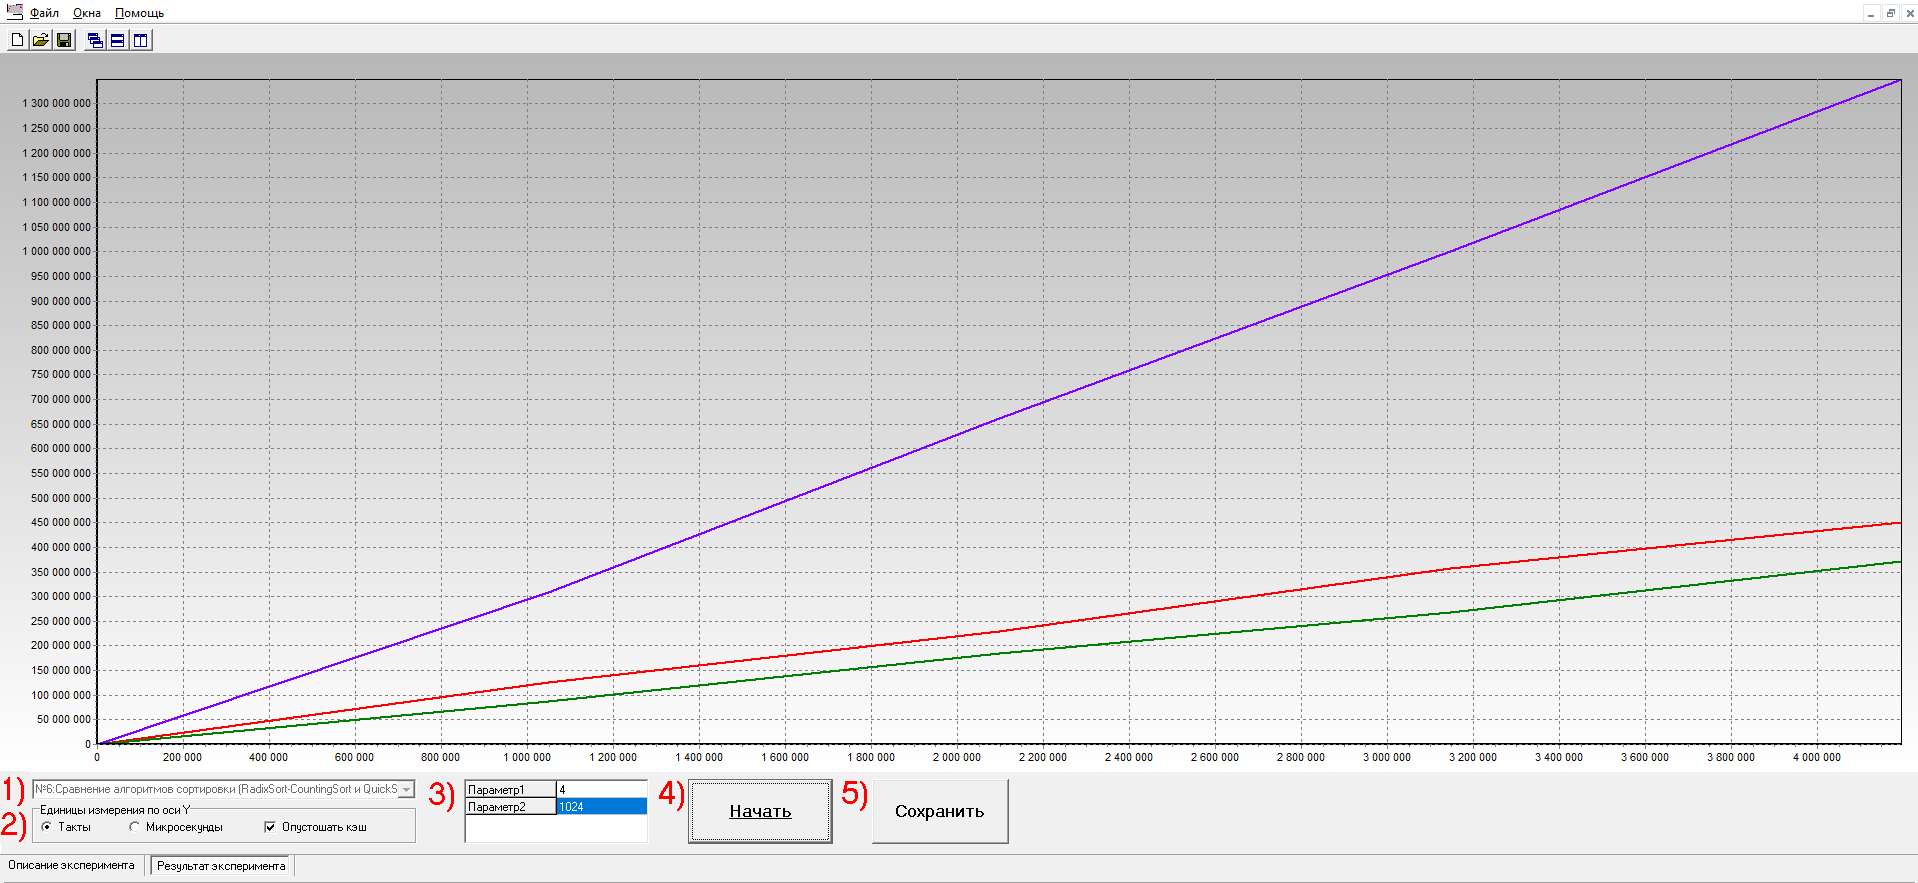
\includegraphics[width=170mm]{./img/6.png}
    \caption{Эксперимент 5: Сравнение алгоритмов сортировки}
\end{figure}

\begin{figure}[ht!]
    \centering
    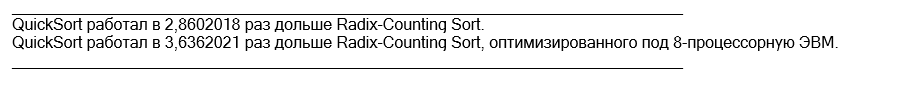
\includegraphics[width=100mm]{./img/06.png}
    \caption{Эксперимент 6: Результаты\label{res_06}}
\end{figure}

Как видно на рисунке \ref{res_06}, QuickSort работал примерно в 2,86 раз дольше Radix-Counting Sort, и QuickSort работал примерно в 3,64 раз дольше Radix-Counting Sort, оптимизированного под 8-процессорную ЭВМ.

\section{Вывод}
Исходя из полученных результатов, можно сделать вывод, что существуют сортировки, которые работают быстрее QuickSort. Также данные сортировки можно дополнительно оптимизировать.